\documentclass[manuscript, review, anonymous, screen]{acmart}


\IfFileExists{upquote.sty}{\usepackage{upquote}}{}
\IfFileExists{microtype.sty}{% use microtype if available
  \usepackage[]{microtype}
  \UseMicrotypeSet[protrusion]{basicmath} % disable protrusion for tt fonts
}{}
\makeatletter
\@ifundefined{KOMAClassName}{% if non-KOMA class
  \IfFileExists{parskip.sty}{%
    \usepackage{parskip}
  }{% else
    \setlength{\parindent}{0pt}
    \setlength{\parskip}{6pt plus 2pt minus 1pt}}
}{% if KOMA class
  \KOMAoptions{parskip=half}}
\makeatother

%%
%% This is file `sample-manuscript.tex',
%% generated with the docstrip utility.
%%
%% The original source files were:
%%
%% samples.dtx  (with options: `manuscript')
%% 
%% IMPORTANT NOTICE:
%% 
%% For the copyright see the source file.
%% 
%% Any modified versions of this file must be renamed
%% with new filenames distinct from sample-manuscript.tex.
%% 
%% For distribution of the original source see the terms
%% for copying and modification in the file samples.dtx.
%% 
%% This generated file may be distributed as long as the
%% original source files, as listed above, are part of the
%% same distribution. (The sources need not necessarily be
%% in the same archive or directory.)
%%
%%
%% Commands for TeXCount
%TC:macro \cite [option:text,text]
%TC:macro \citep [option:text,text]
%TC:macro \citet [option:text,text]
%TC:envir table 0 1
%TC:envir table* 0 1
%TC:envir tabular [ignore] word
%TC:envir displaymath 0 word
%TC:envir math 0 word
%TC:envir comment 0 0
%%
%%
%% The first command in your LaTeX source must be the \documentclass command.


% Options for packages loaded elsewhere
\PassOptionsToPackage{unicode}{hyperref}
\PassOptionsToPackage{hyphens}{url}
\PassOptionsToPackage{dvipsnames,svgnames,x11names}{xcolor}

\IfFileExists{bookmark.sty}{\usepackage{bookmark}}{\usepackage{hyperref}}

%% PANDOC PREAMBLE BEGINS


\providecommand{\tightlist}{%
  \setlength{\itemsep}{0pt}\setlength{\parskip}{0pt}}\usepackage{longtable,booktabs,array}
\usepackage{calc} % for calculating minipage widths
% Correct order of tables after \paragraph or \subparagraph
\usepackage{etoolbox}
\makeatletter
\patchcmd\longtable{\par}{\if@noskipsec\mbox{}\fi\par}{}{}
\makeatother
% Allow footnotes in longtable head/foot
\IfFileExists{footnotehyper.sty}{\usepackage{footnotehyper}}{\usepackage{footnote}}
\makesavenoteenv{longtable}
\usepackage{graphicx}
\makeatletter
\def\maxwidth{\ifdim\Gin@nat@width>\linewidth\linewidth\else\Gin@nat@width\fi}
\def\maxheight{\ifdim\Gin@nat@height>\textheight\textheight\else\Gin@nat@height\fi}
\makeatother
% Scale images if necessary, so that they will not overflow the page
% margins by default, and it is still possible to overwrite the defaults
% using explicit options in \includegraphics[width, height, ...]{}
\setkeys{Gin}{width=\maxwidth,height=\maxheight,keepaspectratio}
% Set default figure placement to htbp
\makeatletter
\def\fps@figure{htbp}
\makeatother

\usepackage{booktabs}
\usepackage{longtable}
\usepackage{array}
\usepackage{multirow}
\usepackage{wrapfig}
\usepackage{float}
\usepackage{colortbl}
\usepackage{pdflscape}
\usepackage{tabu}
\usepackage{threeparttable}
\usepackage{threeparttablex}
\usepackage[normalem]{ulem}
\usepackage{makecell}
\usepackage{xcolor}
\definecolor{mypink}{RGB}{219, 48, 122}
\makeatletter
\makeatother
\makeatletter
\makeatother
\makeatletter
\@ifpackageloaded{caption}{}{\usepackage{caption}}
\AtBeginDocument{%
\ifdefined\contentsname
  \renewcommand*\contentsname{Table of contents}
\else
  \newcommand\contentsname{Table of contents}
\fi
\ifdefined\listfigurename
  \renewcommand*\listfigurename{List of Figures}
\else
  \newcommand\listfigurename{List of Figures}
\fi
\ifdefined\listtablename
  \renewcommand*\listtablename{List of Tables}
\else
  \newcommand\listtablename{List of Tables}
\fi
\ifdefined\figurename
  \renewcommand*\figurename{Figure}
\else
  \newcommand\figurename{Figure}
\fi
\ifdefined\tablename
  \renewcommand*\tablename{Table}
\else
  \newcommand\tablename{Table}
\fi
}
\@ifpackageloaded{float}{}{\usepackage{float}}
\floatstyle{ruled}
\@ifundefined{c@chapter}{\newfloat{codelisting}{h}{lop}}{\newfloat{codelisting}{h}{lop}[chapter]}
\floatname{codelisting}{Listing}
\newcommand*\listoflistings{\listof{codelisting}{List of Listings}}
\makeatother
\makeatletter
\@ifpackageloaded{caption}{}{\usepackage{caption}}
\@ifpackageloaded{subcaption}{}{\usepackage{subcaption}}
\makeatother
\makeatletter
\@ifpackageloaded{tcolorbox}{}{\usepackage[skins,breakable]{tcolorbox}}
\makeatother
\makeatletter
\@ifundefined{shadecolor}{\definecolor{shadecolor}{rgb}{.97, .97, .97}}
\makeatother
\makeatletter
\makeatother
\makeatletter
\makeatother
%% PANDOC PREAMBLE ENDS

\setlength{\parindent}{10pt}
\setlength{\parskip}{0pt}

\hypersetup{
  pdftitle={Further Investigating the Effects of Point Size and Contrast on Correlation Perception in Scatterplots},
  pdfauthor={Gabriel Strain; Andrew J. Stewart; Paul Warren; Caroline Jay},
  colorlinks=true,
  linkcolor={blue},
  filecolor={Maroon},
  citecolor={Blue},
  urlcolor={red},
  pdfcreator={LaTeX via pandoc, via quarto}}

%% \BibTeX command to typeset BibTeX logo in the docs
\AtBeginDocument{%
  \providecommand\BibTeX{{%
    Bib\TeX}}}

%% Rights management information.  This information is sent to you
%% when you complete the rights form.  These commands have SAMPLE
%% values in them; it is your responsibility as an author to replace
%% the commands and values with those provided to you when you
%% complete the rights form.
\setcopyright{acmcopyright}
\copyrightyear{2018}
\acmYear{2018}
\acmDOI{XXXXXXX.XXXXXXX}

%% These commands are for a PROCEEDINGS abstract or paper.
\acmConference[CHI]{Make sure to enter the correct conference title from
your rights confirmation emai}{June 03--05, 2018}{Woodstock, NY}
\acmPrice{15.00}
\acmISBN{978-1-4503-XXXX-X/18/06}

%% Submission ID.
%% Use this when submitting an article to a sponsored event. You'll
%% receive a unique submission ID from the organizers
%% of the event, and this ID should be used as the parameter to this command.
%%\acmSubmissionID{123-A56-BU3}

%%
%% For managing citations, it is recommended to use bibliography
%% files in BibTeX format.
%%
%% You can then either use BibTeX with the ACM-Reference-Format style,
%% or BibLaTeX with the acmnumeric or acmauthoryear sytles, that include
%% support for advanced citation of software artefact from the
%% biblatex-software package, also separately available on CTAN.
%%
%% Look at the sample-*-biblatex.tex files for templates showcasing
%% the biblatex styles.
%%

%%
%% The majority of ACM publications use numbered citations and
%% references.  The command \citestyle{authoryear} switches to the
%% "author year" style.
%%
%% If you are preparing content for an event
%% sponsored by ACM SIGGRAPH, you must use the "author year" style of
%% citations and references.
%% Uncommenting
%% the next command will enable that style.
%%\citestyle{acmauthoryear}


%% end of the preamble, start of the body of the document source.
\begin{document}


%%
%% The "title" command has an optional parameter,
%% allowing the author to define a "short title" to be used in page headers.
\title[Size, Contrast, and Scatterplots]{Further Investigating the
Effects of Point Size and Contrast on Correlation Perception in
Scatterplots}

%%
%% The "author" command and its associated commands are used to define
%% the authors and their affiliations.
%% Of note is the shared affiliation of the first two authors, and the
%% "authornote" and "authornotemark" commands
%% used to denote shared contribution to the research.


  \author{Gabriel Strain}
  \orcid{0000-0002-4769-9221}
            \affiliation{%
                  \institution{Department of Computer Science, Faculty
of Science and Engineering, University of Manchester}
                          \streetaddress{Oxford Road}
                          \city{Manchester}
                                  \country{United Kingdom}
                          \postcode{M13 9PL}
              }
        \author{Andrew J. Stewart}
  
            \affiliation{%
                  \institution{Department of Computer Science, Faculty
of Science and Engineering, University of Manchester}
                          \streetaddress{Oxford Road}
                          \city{Manchester}
                                  \country{United Kingdom}
                          \postcode{M13 9PL}
              }
        \author{Paul Warren}
  
            \affiliation{%
                  \institution{Division of Psychology, Communication and
Human Neuroscience, School of Health Sciences, Faculty of Biology,
Medicine, and Health, University of Manchester}
                          \streetaddress{Oxford Road}
                          \city{Manchester}
                                  \country{United Kingdom}
                          \postcode{M13 9PL}
              }
        \author{Caroline Jay}
  
            \affiliation{%
                  \institution{Department of Computer Science, Faculty
of Science and Engineering, University of Manchester}
                          \streetaddress{Oxford Road}
                          \city{Manchester}
                                  \country{United Kingdom}
                          \postcode{M13 9PL}
              }
      
\renewcommand{\shortauthors}{Strain et al.}

%% By default, the full list of authors will be used in the page
%% headers. Often, this list is too long, and will overlap
%% other information printed in the page headers. This command allows
%% the author to define a more concise list
%% of authors' names for this purpose.
%\renewcommand{\shortauthors}{Trovato et al.}
%%  
%% The abstract is a short summary of the work to be presented in the
%% article.
\begin{abstract}
Abstract goes here    
\end{abstract}

%%
%% The code below is generated by the tool at http://dl.acm.org/ccs.cfm.
%% Please copy and paste the code instead of the example below.
%%
\begin{CCSXML}
<ccs2012>
 <concept>
  <concept_id>10010520.10010553.10010562</concept_id>
  <concept_desc>Computer systems organization~Embedded systems</concept_desc>
  <concept_significance>500</concept_significance>
 </concept>
 <concept>
  <concept_id>10010520.10010575.10010755</concept_id>
  <concept_desc>Computer systems organization~Redundancy</concept_desc>
  <concept_significance>300</concept_significance>
 </concept>
 <concept>
  <concept_id>10010520.10010553.10010554</concept_id>
  <concept_desc>Computer systems organization~Robotics</concept_desc>
  <concept_significance>100</concept_significance>
 </concept>
 <concept>
  <concept_id>10003033.10003083.10003095</concept_id>
  <concept_desc>Networks~Network reliability</concept_desc>
  <concept_significance>100</concept_significance>
 </concept>
</ccs2012>
\end{CCSXML}

\ccsdesc[500]{Computer systems organization~Embedded systems}
\ccsdesc[300]{Computer systems organization~Redundancy}
\ccsdesc{Computer systems organization~Robotics}
\ccsdesc[100]{Networks~Network reliability}

%%
%% Keywords. The author(s) should pick words that accurately describe
%% the work being presented. Separate the keywords with commas.
\keywords{correlation, scatterplot, perception, crowdsourced}


%%
%% This command processes the author and affiliation and title
%% information and builds the first part of the formatted document.
\maketitle

\setlength{\parskip}{-0.1pt}

\hypertarget{introduction}{%
\section{Introduction}\label{introduction}}

\begin{itemize}
\tightlist
\item
  why study scatterplots?
\item
  correlation perception
\end{itemize}

We have previously demonstrated the potential for changes in point size
and point contrast to bias peoples' estimates of correlation in
scatterplots. Lowering the size and contrast of scatterplot points as
they move further from the regression line partially corrects for the
underestimation bias described above. We have hypothesized in our
previous work that what is driving the changes in correlation estimation
that we have seen is an increase in spatial uncertainty at the edges of
the scatterplot relative to the center, which itself drives a reduction
in the perceived width of the probability distribution said scatterplot
represents. As part of our ongoing effort to tune scatterplots for more
accurate correlation perception, our next step is to combine our point
size and contrast manipulations. In the present study we hypothesize
that; an increased reduction in correlation estimation error will be
observed when congruent non-linear functions are used; the use of
congruent inverted conditions will produce the least accurate estimates
of correlation; and that owing to the greater strength of the size
channel observed in \citet{strain_2023b}, there will be a significant
difference in correlation estimates between the two incongruent
conditions.

\hypertarget{sec-related-work}{%
\section{Related Work}\label{sec-related-work}}

\hypertarget{sec-testing-corr-percept}{%
\subsection{Testing Correlation
Perception}\label{sec-testing-corr-percept}}

\hypertarget{sec-drivers}{%
\subsection{Drivers of Correlation Perception}\label{sec-drivers}}

\hypertarget{sec-transparency-and-contrast}{%
\subsection{Transparency and
Contrast}\label{sec-transparency-and-contrast}}

Changing the contrast of scatterplot points is standard practice to deal
with issues of overplotting or clutter (\citet{matejka_2015};
\citet{bertini_2004}); scatterplots with very large numbers of points,
especially with high degrees of overlap, suffer from low
individual-point visibility caused by high point density. Lowering the
contrast of all points addresses this, and makes data trends and
distributions easier to see and interpret. Previous work has found that
lowering the contrast of \emph{all} scatterplot points relative to the
background can increase the level of underestimation error relative to
full contrast, and that lowering point contrast \emph{as a function of
distance from the regression line} is able to bias correlation estimates
upwards to partially correct for the underestimation bias
(\citet{strain_2023}). The balance of evidence points towards an
uncertainty-based mechanism for these effects. Lower contrast can
increase error in positional judgements (\citet{wehrhahn_1990}), can
result in greater uncertainty in speed perception
(\citet{champion_2017})

\begin{itemize}
\item
  formalising contrast
\item
  ggplot etc
\item
  use of contrast floor
\item
  rehash contrast paper main points about contrast/alpha
\item
  explain luminance, alpha, etc
\item
  clarify use of alpha = 0.2 floor
\end{itemize}

\hypertarget{sec-point-size}{%
\subsection{Point Size}\label{sec-point-size}}

\begin{itemize}
\tightlist
\item
  interplay between size and spatial uncertainty
\item
  hype up how strong the size effect was last time
\end{itemize}

\hypertarget{sec-methods}{%
\section{Methodology}\label{sec-methods}}

\hypertarget{crowdsourcing}{%
\subsection{Crowdsourcing}\label{crowdsourcing}}

\begin{itemize}
\tightlist
\item
  issues with crowdsourcing
\item
  how those issues were solved
\item
  why did we choose to crowdsource
\end{itemize}

Discussions about the transparency, contrast, and luminance is
inherently difficult within the context of online, crowdsourced
experimental work. While the ease, low-cost, and resilience to different
viewing contexts afforded to us by such work is advantageous, we must
also consider the impact on our ability to precisely describe the
experimental stimuli.

\hypertarget{sec-open-research}{%
\subsection{Open Research}\label{sec-open-research}}

Both experiments were conducted according to the principles of open and
reproducible research. All data and analysis code are available at
(repository link removed for anon). This repository contains
instructions for building a docker image to fully reproduce the
computational environment used . This allows for full replications of
stimuli, analysis, and the paper itself. Ethical approval for both
experiments was granted by (removed for anon). Hypotheses and analysis
plans were pre-registered with the OSF (links removed for anon).

\hypertarget{sec-scatter-gen}{%
\subsection{Scatterplot Generation}\label{sec-scatter-gen}}

The data used to generate the scatterplots were identical to that used
in our previous work \citep{strain_2023, strain_2023b}. 45 scatterplot
datasets were generated corresponding to 45 \emph{r} values uniformly
distributed between 0.2 and 0.99, as there is evidence that very little
correlation is perceived below \emph{r} = 0.2
\citep{strahan_1978, bobko_1979, cleveland_1982}. Using so many values
for \emph{r} allows us to paint a broader picture of people's
perceptions than work using fewer values. Scatterplot points were
generated based on bivariate normal distributions with standard
deviations of 1 in each direction. Each scatterplot had a 1:1 aspect
ratio, was generated as a 1000*1000 pixel .png image, and was scaled up
or down according to a participant's monitor such that they always
occupied the same visual proportion. We used equation 1 to map residuals
to size and contrast values.

\begin{equation}
  point_{size/contrast} = 1 - 0.25^{residual}
\end{equation}

In experiment 1, we used 2x2 combinations of this equation in standard
and inverted forms. Scatterplot examples can be seen in
Figure~\ref{fig-examples}. In experiment 2 we fine tune this equation,
adding the objective \emph{r} value and the previously observed biases
into the equation in order to flatten the underestimation curve.

\hypertarget{sec-gen-modelling}{%
\subsection{Modelling}\label{sec-gen-modelling}}

In both experiments we use linear mixed effects models to model the
relationships between our independent variables (the combination of size
and contrast decay conditions in experiment 1, and the use of the tuned
manipulation in experiment 2) and participants' errors in correlation
estimates. Models such as these allow us to compare differences in our
IVs across the full range of participant responses, as opposed to
relying purely on aggregate data, as in ANOVA. These models also afford
us the ability to include random effects for participants and items. As
per our pre-registrations we preferred maximal models, including random
intercepts and slopes for participants and items. The structures of
these models was identified using the \textbf{buildmer} package in R
(version xx, \citet{voeten_buildmer}). This package takes a maximal
random effects structure and then identifies the most complex model that
converges, dropping random effects terms that fail to explain a
significant amount of variance.

\hypertarget{sec-VT}{%
\subsection{Point Visibility Testing}\label{sec-VT}}

It is key that our manipulations do not remove data from the
scatterplot. In order to ensure that our points were visible, we
included visual threshold testing. Participants viewed six scatterplots
that were made up of a certain number of points. These points were of
the same size and contrast as the smallest and lowest contrast points to
be used in that experiment. Participants were asked to enter in a
textbox how many points were present. In experiment 1, participants
scored an average of 74.89\% (\(SD\) = 32.25). Despite our use of the
contrast floor detailed in Section~\ref{sec-transparency-and-contrast},
it is clear that some of our small, low contrast points were not
reliably visible, most likely due to low contrast between the point and
background, as our previous work (strain\_2023b) found point visibility
invariant to size. We suggest this is due to differences in monitors
between participants. In reality this contrast floor would need to
calibrated on a per-monitor basis. Figure~\ref{fig-VT-hist} shows
distributions of participants' performances on the visual threshold
tests. We also include performance as fixed effects in experimental
models in Section~\ref{sec-results} and

\begin{figure}

{\centering 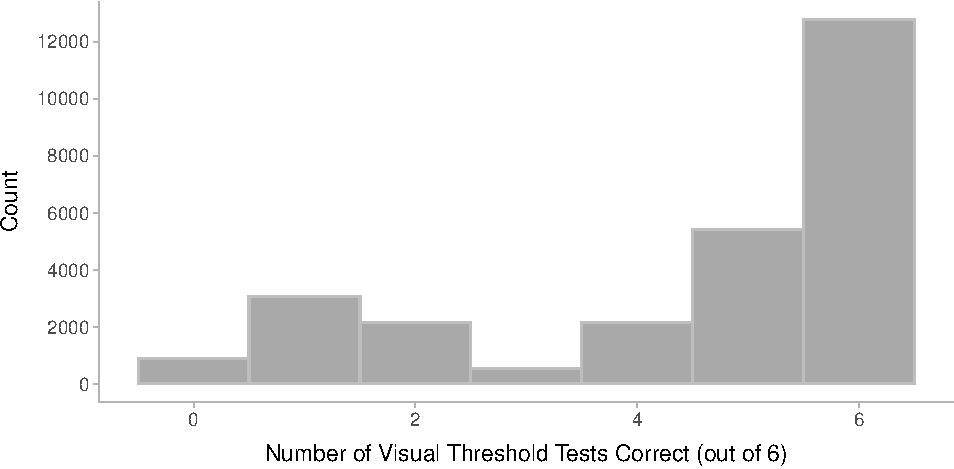
\includegraphics{size_and_contrast_new_files/figure-pdf/fig-VT-hist-1.pdf}

}

\caption{\label{fig-VT-hist}Histograms of visual threshold testing
performance for experiment 1 (L) and experiment 2 (R).}

\end{figure}

\hypertarget{sec-dot-pitch}{%
\subsection{Dot Pitch}\label{sec-dot-pitch}}

We employed a method for obtaining the dot pitch of participants'
monitors (\citet{screenscale}). Combining this with monitor resolution
information allows us to calculate the physical on-screen size of
scatterplot points. Participants were asked to hold a standard size
credit/ debit/ID card (ISO/IEC 7810 ID-1) up to their screen and resize
an on-screen card until the two matched. We assumed a widescreen 16:9
aspect ratio and calculated dot pitch based on these measurements. Mean
dot pitch in experiment 1 was 0.34 (\(SD\) = 0.05) and xx in experiment
2. We include analyses with dot pitch as a fixed effect below.

\hypertarget{sec-gen-procedure}{%
\subsection{Procedure}\label{sec-gen-procedure}}

Both experiments were built using PsychoPy (\citet{pierce_2019}) and
hosted on Pavlovia.org. Participants were only permitted to complete the
experiments on a desktop or laptop computer. Each participant was first
shown the participant information sheet and provided consent through key
presses in response to consent statements. They were asked to provide
their age in a free text box, followed by their gender identity.
Participants completed the 5-item Subjective Graph Literacy test
(\citet{garcia_2016}), followed by the visual threshold task described
in Section~\ref{sec-VT} and the screen scale task described in
Section~\ref{sec-dot-pitch}. Participants were given instructions, and
were then shown examples of scatterplots with correlations of \emph{r} =
0.2, 0.5, 0.8, and 0.95, as piloting of a previous experiment indicated
some of the lay population may be unfamiliar with the visual character
of scatterplots. Section~\ref{sec-results} contains further discussion
of the potential training effects of this. Two practice trials were
given before the experiment began. Participants worked through a
randomly presented series of 180 experimental trials (90 in experiment
2?) and were asked to use a slider to estimate correlation to 2 decimal
places. Visual masks preceded each scatterplot. Interspersed were 6
attention check trials which explicitly asked participants to ignore the
scatterplot and set the slider to 0 or 1.

\hypertarget{sec-participants}{%
\subsection{Participants}\label{sec-participants}}

150 participants were recruited using the Prolific.co platform. Normal
to corrected-to-normal vision and English fluency were required for
participation. To ensure high quality data, and in accordance with
guidelines published in \citet{peer_2021}, participants were required to
have successfully completed a minimum of 100 studies on Prolific. In
addition, participants who had completed any of our previous studies
into correlation estimation in scatterplots \citep[and a previous
pre-study]{strain_2023, strain_2023b} were prevented from participating.

Data were collected from 158 participants. 8 failed more than 2 our of 6
attention check questions, and, as per pre-registration stipulations,
were rejected from the study. Data from the remaining 150 participants
were included in the full analysis (50.7\% male, 48.7\% female, and
0.7\% non-binary). Participants mean age was 30.6 (\emph{SD} = 8.6).
Participants' mean graph literacy score was 22.5 (\emph{SD} = 3.5). The
average time taken to complete the experiment was 37 minutes (\emph{SD}
= 12.3).

\hypertarget{sec-design}{%
\subsection{Design}\label{sec-design}}

We used a fully repeated-measures 2*2 factorial design in experiment 1.
Each participant saw each combination of size and contrast decay
condition plots for a total of 180 experimental items. Participants
viewed these experimental items, along with 6 attention check items, in
a fully randomized order. Examples of experimental items can be seen in
Figure~\ref{fig-examples}.

\begin{figure}

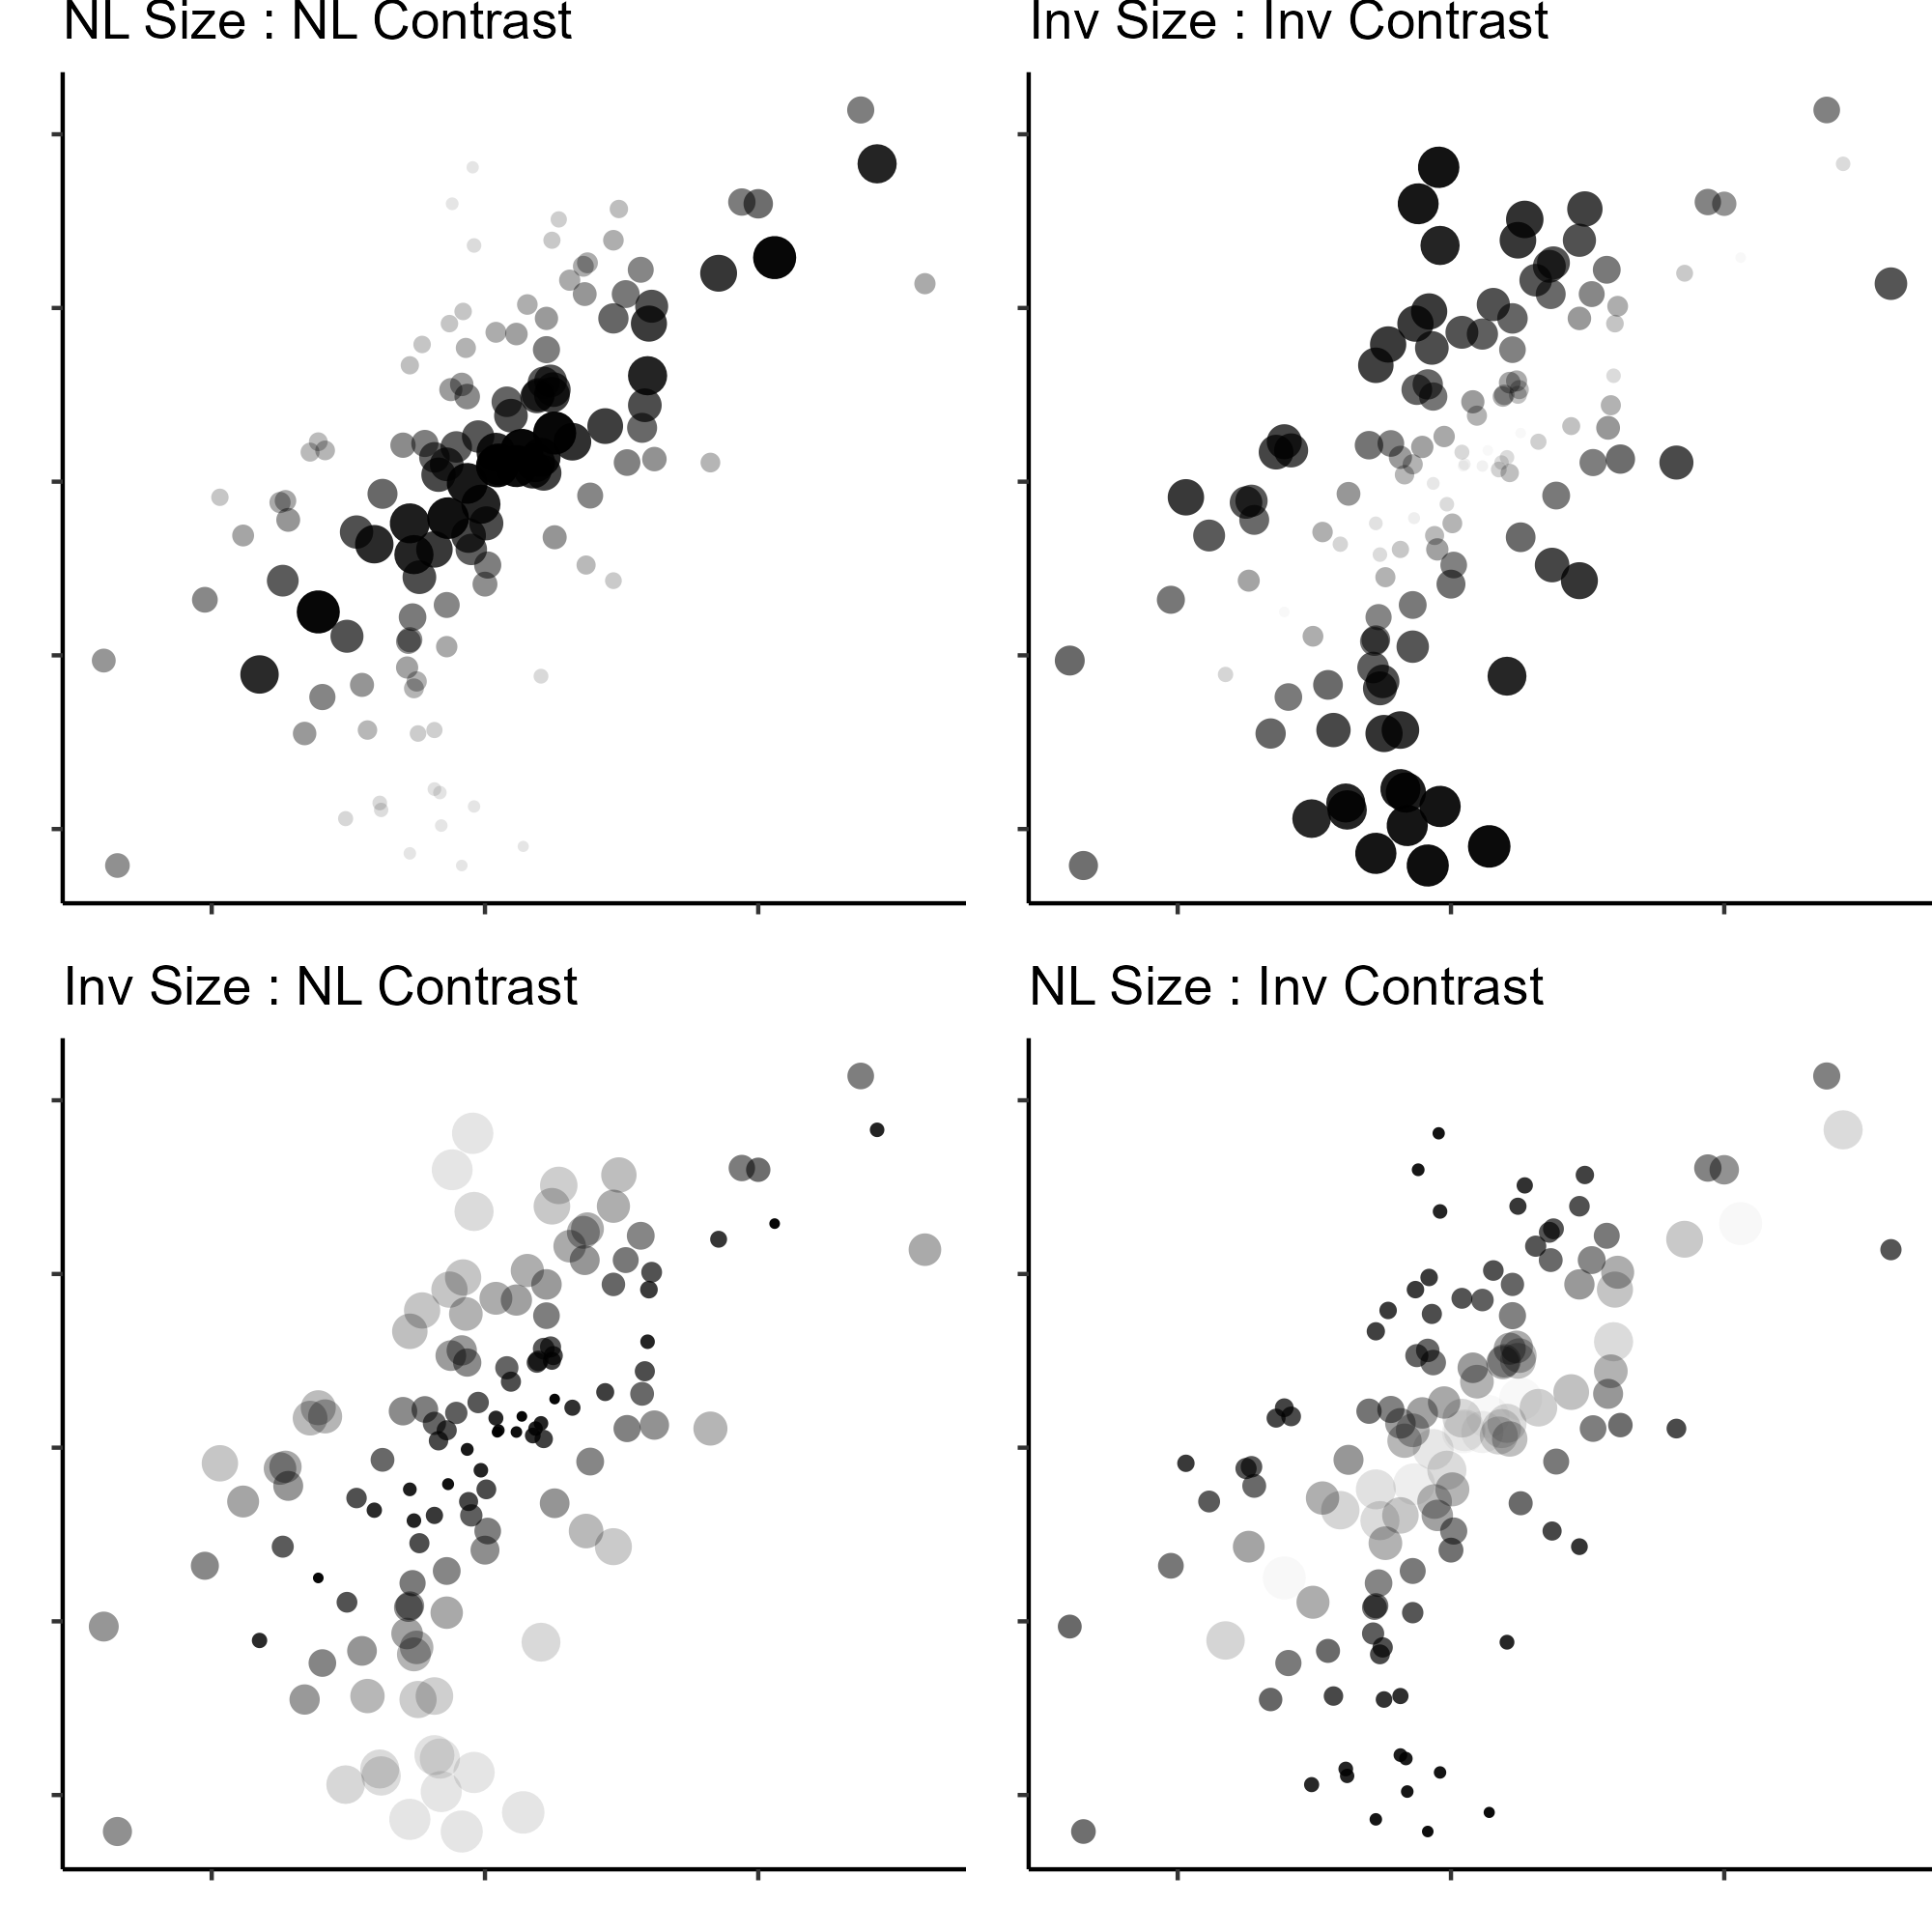
\includegraphics[width=0.5\textwidth,height=\textheight]{images/examples.png} \hfill{}

\caption{\label{fig-examples}Examples of the experimental items used. NL
= non-linear decay, Inv = inverted decay.}

\end{figure}

\hypertarget{sec-results}{%
\section{Results}\label{sec-results}}

Our first two hypotheses were fully supported in this experiment. The
combination of non-linear size and contrast decay functions produced the
most accurate estimates of correlation, although this also resulted in a
large correlation overestimation for many values of \emph{r} (see
Figure~\ref{fig-diff-error-bars-plot}). Our second hypothesis was also
supported; the combination of inverted size and inverted contrast decay
conditions produced the least accurate estimates of correlation. We
found no support for our third hypothesis; there was no significant
difference in correlation estimates for non-linear size/inverted
contrast decay plots and inverted size/non-linear contrast decay plots
(Z = -2.26, \emph{p} = .11), however we did find a significant
interaction effect that provides evidence that the size decay function
was stronger with regards to biasing people's estimates of correlation.

\hypertarget{tbl-sig}{}
\begin{table}
\caption{\label{tbl-sig}Significances of fixed effects and interaction for experiment 1. }\tabularnewline

\centering
\begin{tabular}{lrrrrl}
\toprule
  & Estimate & Standard Error & df & t-value & p\\
\midrule
(Intercept) & 0.08 & 0.013 & 103.32 & 6.27 & <0.001\\
Size Decay & -0.14 & 0.005 & 148.39 & -25.77 & <0.001\\
Contrast Decay & 0.12 & 0.002 & 26327.21 & 63.71 & <0.001\\
Size Decay x Contrast Decay & 0.15 & 0.004 & 26327.13 & 38.47 & <0.001\\
\bottomrule
\end{tabular}
\end{table}

All analyses were conducted using R (version 4.3.1). Deviation coding
was used for each of the experimental factors. We used the
\textbf{buildmer} and \textbf{lme4} packages to build a linear mixed
effects model where the difference between objective and rated r value
was predicted by the size and contrast decay conditions used. A
likelihood ratio test revealed that the model including point size and
contrast decay conditions as fixed effects explained significantly more
variance than the null (\(\chi^2\)(3) = 5,286.81, \emph{p} \textless{}
.001). There were significant fixed effects of size decay and contrast
decay conditions, as well as a significant interaction between the two.
Table~\ref{tbl-sig} shows a summary of the model statistics. The
experimental model has random intercepts for items and participants, and
a random slope for the size decay factor with regards to participants.

\begin{figure}

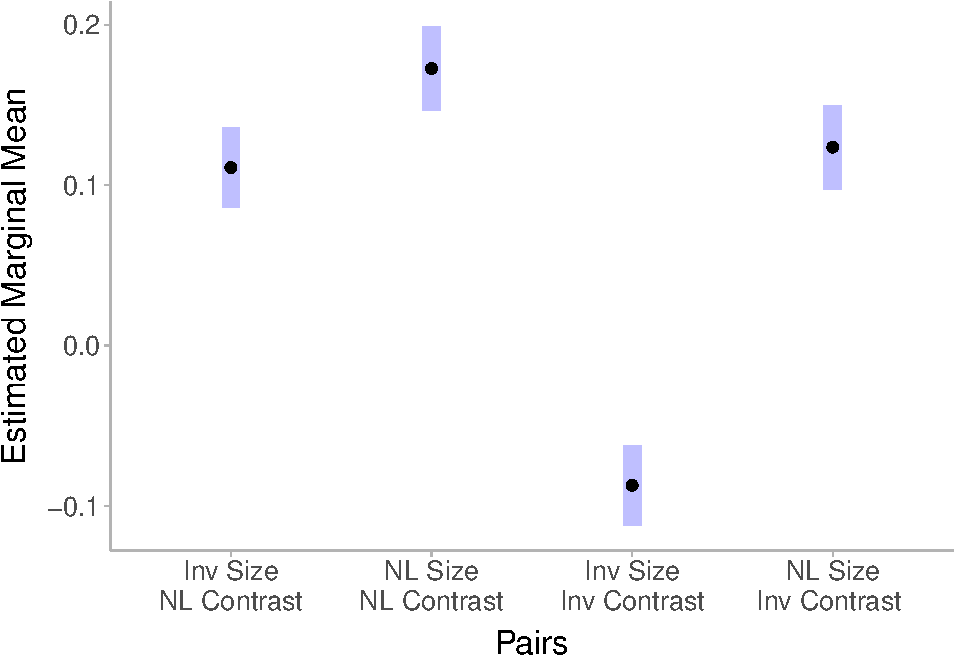
\includegraphics[width=0.5\textwidth,height=\textheight]{size_and_contrast_new_files/figure-pdf/fig-emm-plot-1.pdf} \hfill{}

\caption{\label{fig-emm-plot}\textbf{?(caption)}}

\end{figure}

\begin{figure}

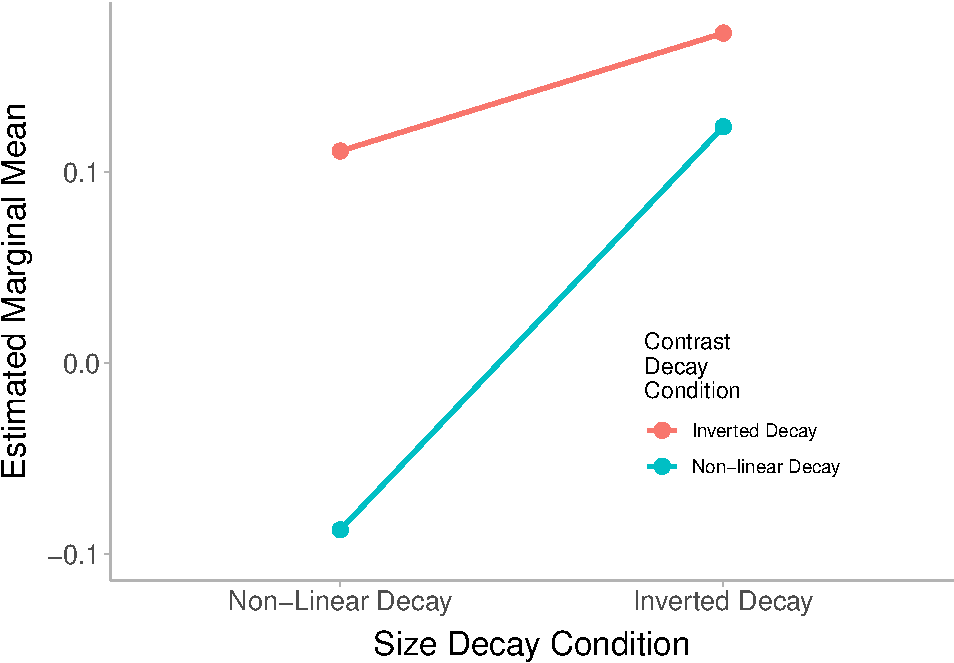
\includegraphics[width=0.5\textwidth,height=\textheight]{size_and_contrast_new_files/figure-pdf/fig-interaction-plot-1.pdf} \hfill{}

\caption{\label{fig-interaction-plot}Interaction plot showing the
moderating effect of encoding channel on decay orientation.}

\end{figure}

\hypertarget{tbl-contrasts}{}
\begin{table}
\caption{\label{tbl-contrasts}Pairwise comparisons for experiment 1. Our interaction is driven by the
greater strength of the size channel, whether non-linear or inverted
decay functions were used. Note the lack of significance for NL size/Inv
contrast against Inv size/NL contrast comparison. }\tabularnewline

\centering
\begin{tabular}{lrl}
\toprule
Contrast & Z.ratio & p.value\\
\midrule
Non-linear Size x Inverted Contrast <-> Inverted Size x Inverted Contrast & -10.95 & <0.001\\
Non-linear Size x Inverted Contrast <-> Non-Linear Size x Non-linear Contrast & 72.29 & <0.001\\
Non-linear Size x Inverted Contrast <-> Inverted Size x Non-linear Contrast & -2.26 & 0.108\\
Inverted Size x Inverted Contrast <-> Non-linear Size x Non-linear Contrast & 46.13 & <0.001\\
Inverted Size x Inverted Contrast <-> Inverted Size x Non-linear Contrast & 17.84 & <0.001\\
\addlinespace
Non-linear Size x Non-linear Contrast <-> Inverted Size x Non-linear Contrast & -37.44 & <0.001\\
\bottomrule
\end{tabular}
\end{table}

The \textbf{emmeans} (cite) package was used to run pairwise
comparisons. Figure~\ref{fig-emm-plot} shows estimated marginal means
for each combination of factors, and Figure~\ref{fig-interaction-plot}
shows the form the interaction takes. The interaction is driven by there
being a greater difference in estimates between NL and inverted size
decay conditions when the contrast decay condition is held as
non-linear, as opposed to when it is inverted. This is parsimonious with
our previous work demonstrating the greater capacity of the size
encoding channel to bias participants' estimates of \emph{r}
(\citet{strain_2023b}), and our findings that the inverted channel is
generally weaker at biasing correlation in the opposite direction
(\citet{strain_2023}; \citet{strain_2023b}). Table~\ref{tbl-contrasts}
shows statistics for pairwise comparisons.

\begin{figure}

{\centering 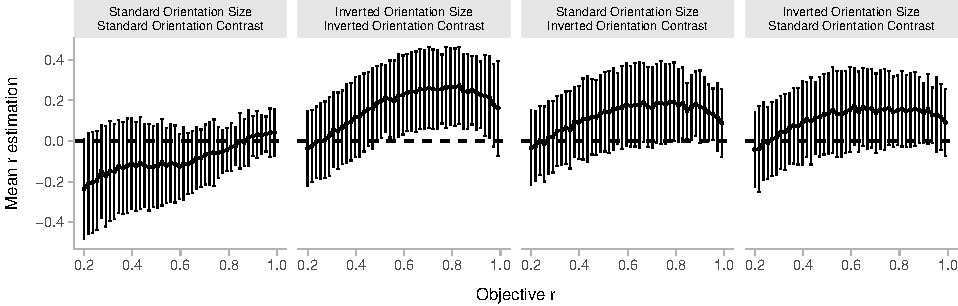
\includegraphics[width=1\textwidth,height=\textheight]{size_and_contrast_new_files/figure-pdf/fig-diff-error-bars-plot-1.pdf}

}

\caption{\label{fig-diff-error-bars-plot}Plots showing how participants'
correlation estimation errors change as a function of the \emph{r} value
for each combination of size and contrast decay factors.}

\end{figure}

We find no effects of graph literacy (\(\chi^2\)(1) = 3.50, \emph{p} =
.061) or performance on the visual threshold task (\(\chi^2\)(1) = 1.29,
\emph{p} = .257), or dot pitch (\(\chi^2\)(1) = 1.52, \emph{p} = .218)
on participants' errors in correlation estimation.

\hypertarget{sec-discussion}{%
\section{Discussion}\label{sec-discussion}}

Our findings here provide further confirmatory evidence of what has been
found previously with regards to the effects of point size and contrast
manipulations on correlation estimation in scatterplots. Namely, that
while both manipulations have a significant effect, the effect of
changing point sizes is stronger, and that while we can influence
correlation estimates in either direction, standard orientation
manipulations are more powerful than inverted ones. The experiment
described above additionally contributes evidence of a congruency
effect; effects are most strong when there is orientation congruency
between size and contrast manipulations.

The lack of support for our third hypothesis, that there would be a
difference in correlation estimates between incongruent conditions, was
surprising given the greater strength of the size channel relative to
contrast. We take this as evidence that the combination of size and
contrast manipulations is not additive, as we had initially suspected,
which explains the interaction we see here. Integrating the data
collected in the present study with previously collected data
investigating the effects of the size and contrast manipulations in
isolation allows us demonstrate this and to partial out the effects each
manipulation.

\begin{figure}

{\centering 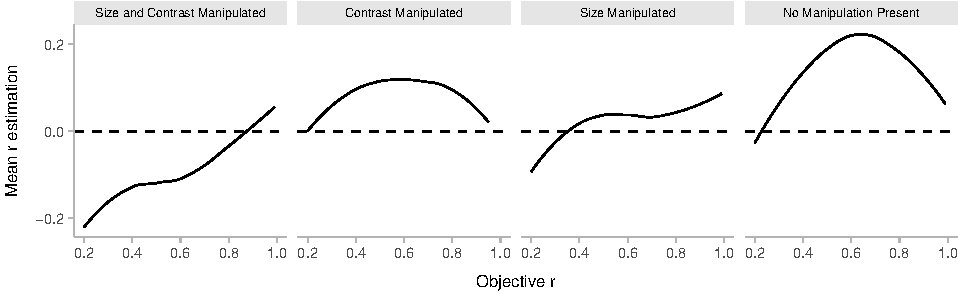
\includegraphics[width=1\textwidth,height=\textheight]{size_and_contrast_new_files/figure-pdf/fig-error-bars-all-exp-1.pdf}

}

\caption{\label{fig-error-bars-all-exp}From left to right, plotting
\emph{r} estimation error against the objective \emph{r} value for the
standard orientation condition in the present study, for standard
orientation size and contrast manipulations in previous work, and for
normal scatterplots averaged over identical conditions in previous work.
Error bars have been left off this plot to make interpretation more
simple.}

\end{figure}

\begin{figure}

{\centering 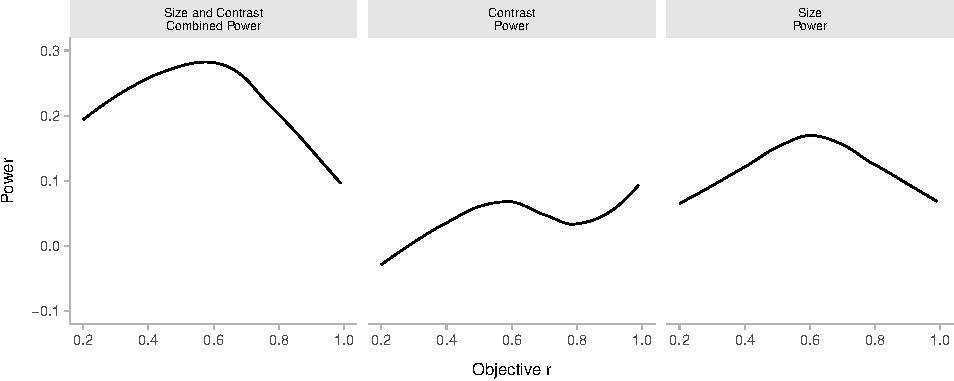
\includegraphics[width=1\textwidth,height=\textheight]{size_and_contrast_new_files/figure-pdf/fig-power-plot-1.pdf}

}

\caption{\label{fig-power-plot}additive\_raw\_pl = observed values for
present study. standard\_curve = no manipulation averaged across all
experiments}

\end{figure}

As can be seen in Figure~\ref{fig-error-bars-all-exp}, combining the
size and contrast manipulations results in an error curve of a mostly
similar shape to that of the size manipulation. The difference that
comes from adding the contrast manipulation lies in the severity of the
effect and the orientation of the curve itself. Transforming the size
underestimation curve from \citet{strain_2023} into the size and
contrast underestimation curve we have found in the present study gives
us some insight into the effect of adding the two manipulations
together.

\begin{figure}

{\centering 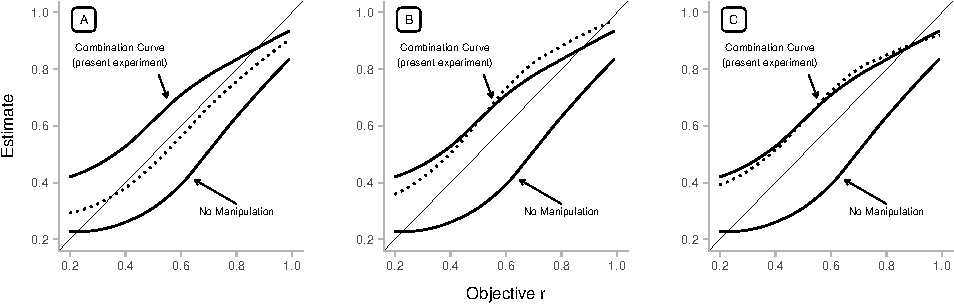
\includegraphics[width=1\textwidth,height=\textheight]{size_and_contrast_new_files/figure-pdf/fig-transformation-1.pdf}

}

\caption{\label{fig-transformation}Transformations required to derive
the Combination Curve observed in the present experiment using the size
and contrast curves from previous work. The dotted line represents the
size curve (A), two times the size curve (B), and two times the size
curve rotated by 6 degrees clockwise.}

\end{figure}

Figure~\ref{fig-transformation} illustrates the transformations we must
do to replicate the results we have found in the present study using
results from previous work (\citet{strain_2023}; \citet{strain_2023b}).
Given the similarity between the shape of the combination curve found in
the present study and that of the size only manipulation found in
\citet{strain_2023b}, we use this as a starting point. Adding the
contrast manipulation has the effect of doubling the power of the size
curve, followed by a change in orientation that can be approximated by a
6\textdegree clockwise rotation. With the knowledge that the addition of
the contrast manipulation can be thought of as doubling and rotating the
size factor, and having worked out \emph{t}, a translation function to
approximate the \(y = x\) optimum estimation line, we are able to
generate the following set of equations. S = size, C = contrast, O =
observed (present study), r = rotation function, t = translation
function.

\begin{equation}
  S + C = O
  r(S + C) = O
  C = S
  r(2S) = O
  tr(2S) = tO
\end{equation}

\bibliographystyle{ACM-Reference-Format}
\bibliography{size-contrast-new.bib}

%% begin pandoc before-bib
%% end pandoc before-bib
%% begin pandoc biblio
%% end pandoc biblio
%% begin pandoc include-after
%% end pandoc include-after
%% begin pandoc after-body
%% end pandoc after-body

\end{document}
\endinput
%%
%% End of file `sample-manuscript.tex'.
